%!TEX root = main.tex

\subsection{An example}

An motivating example is to determine coding or non-coding fragments.

\subsubsection{Baseline approach}


\begin{figure}[htp]
	\centering
	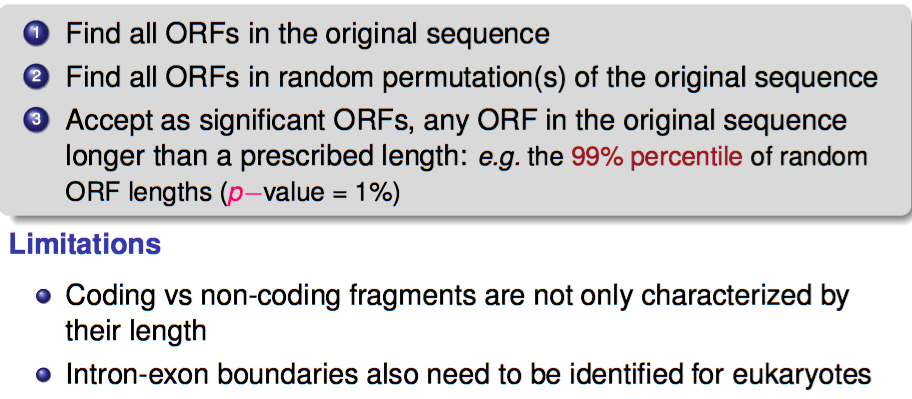
\includegraphics[scale=0.5]{images/17_baseline.png}
\end{figure}

\subsubsection{Alternative approach}

\begin{figure}[htp]
	\centering
	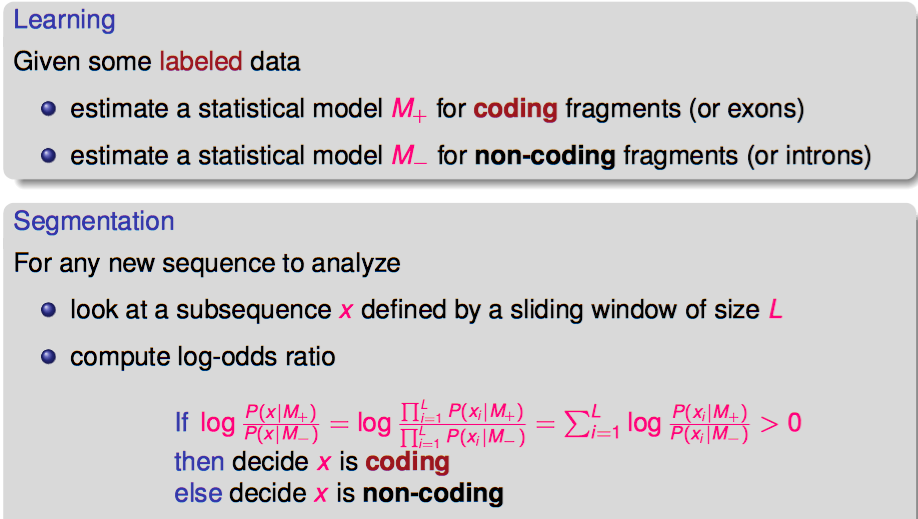
\includegraphics[scale=0.4]{images/18_alt.png}
\end{figure}


\paragraph{Multinomial model}

\begin{center}
  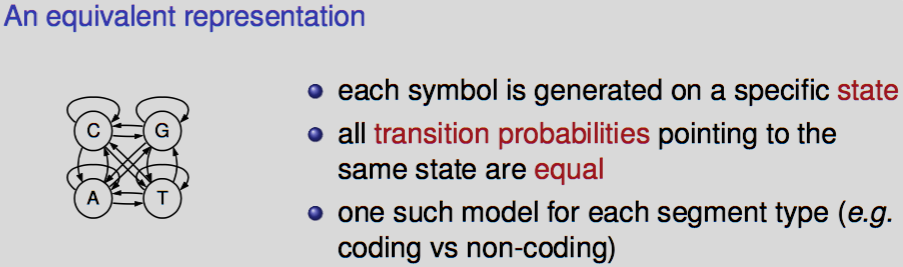
\includegraphics[scale=0.5]{images/19_multi.png}
\captionof{figure}{Two hypothesis: the frequencies are the sames along the different parts of the sequence and each symbol does not depend of surrounding symbols.} 
\end{center}

\newpage
\paragraph{Markov chain}

\begin{center}
	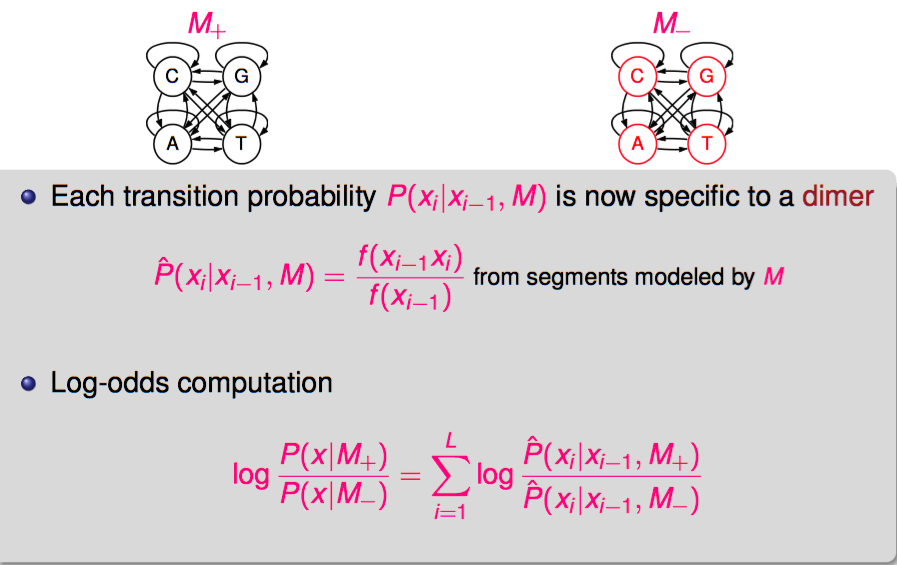
\includegraphics[scale=0.4]{images/20_markov.png}
	\captionof{figure}{First order.}
\end{center}

\begin{center}
	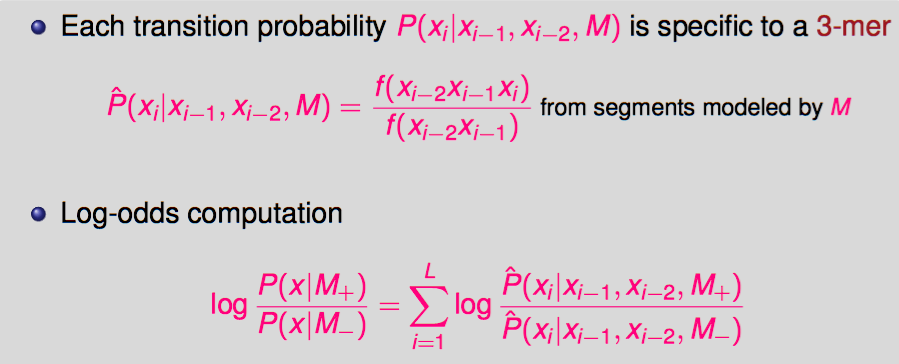
\includegraphics[scale=0.4]{images/21_second.png}
	\captionof{figure}{Second order.}
\end{center}

Limitations of the markov chain approach:
\begin{itemize}
	\item Estimate each MC from well annoted segments;
	\item Gene length variability: sliding window length is arbitrary and we need to find a length that is more relevant: computation expensive;
	\item Eukaryotes: at least three models needed (out of gene, introns, exons).
\end{itemize}
\newpage
\paragraph{Hidden Markov model}

\begin{center}
	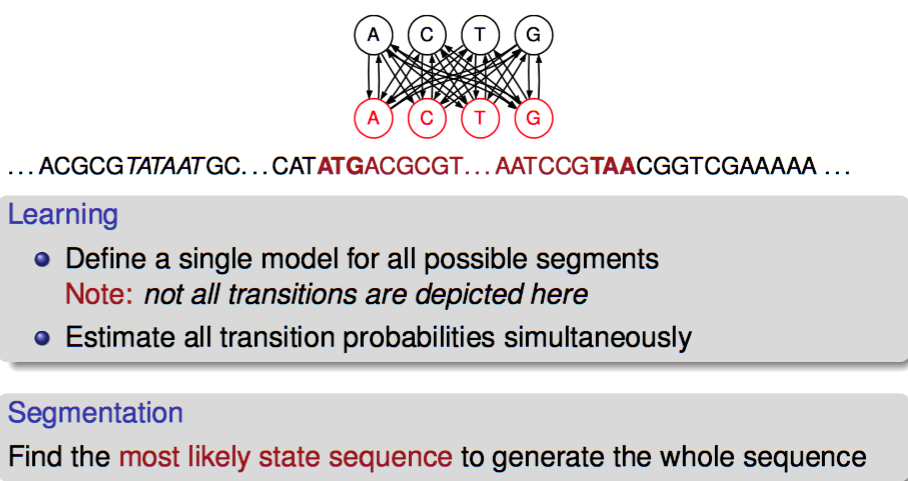
\includegraphics[scale=0.5]{images/22_hmms.png}
	\captionof{figure}{One state for each segment type (coding vs non coding). Transition probabilities, emissions probabilities. States are hidden but their emissions are observed.}
\end{center}

\subsection{Hidden Markov model}

\begin{figure}[htp]
	\centering
	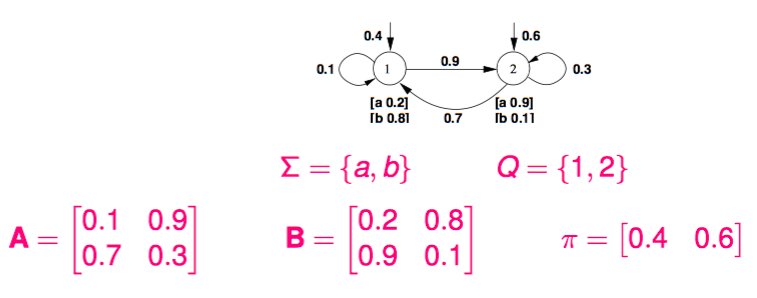
\includegraphics[scale=0.5]{images/24_ex2.png}
\end{figure}

\begin{figure}[htp]
	\centering
	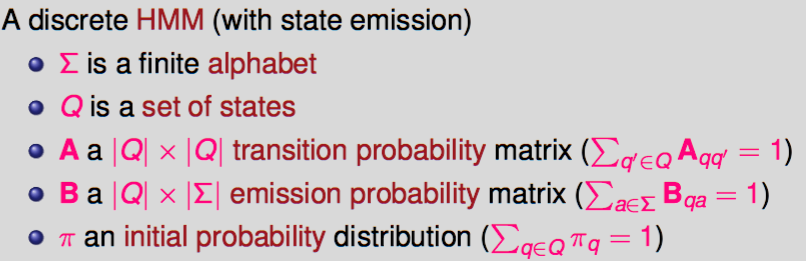
\includegraphics[scale=0.5]{images/23_ex1.png}
	\caption{HMM definition.}
\end{figure}
\newpage
\subsubsection{Path likelihood}

\begin{center}
	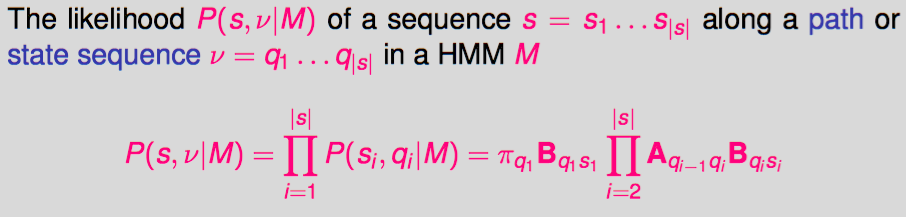
\includegraphics[scale=0.5]{images/25_path.png}
\end{center}

\subsubsection{Probability of generating a sequence}

\begin{figure}[htp]
	\centering
	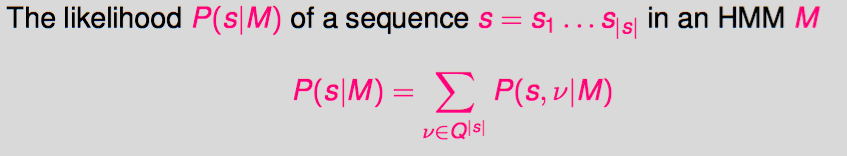
\includegraphics[scale=0.5]{images/26_seq.png}
	\caption{$O(|Q|^{|s|})$ possible state sequences. Q is states and s is sequence.}
\end{figure}

\newpage
\subsubsection{Most likely state sequence}

\begin{figure}[htp]
	\centering
	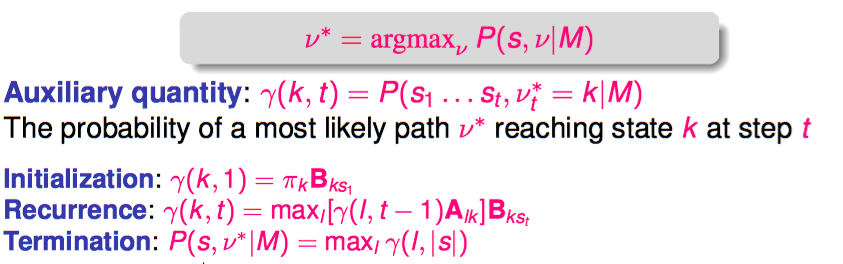
\includegraphics[scale=0.5]{images/27_viterbi.png}
	\caption{Viterbi recurrence.}
\end{figure}

\begin{itemize}
	\item $P(s, v^*)$ gives the probability of the optimal path $v^*$;
	\item Computation are done with log (because too small values);
	\item Complexity: $\Theta(m|s|)$. m is number of HMM transitions;
	\item Path $v^*$ is an alignement between states and words;
	\item $v^*$ can be recovered with the backpointers.
\end{itemize}


\subsubsection{Sequence likelihood}

\begin{figure}[htp]
	\centering
	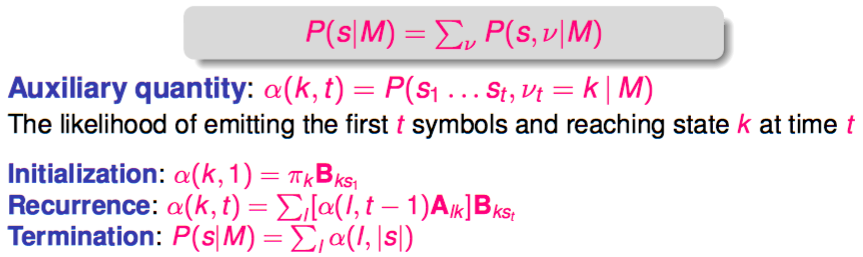
\includegraphics[scale=0.5]{images/28_forward.png}
 	\caption{Forward recurrence, same complexity as viterbi recurrence.}
\end{figure}

\subsection{The learning problem}

Given an HMM structure and several sequences, you must estimate $A$, $B$, $\pi$.


\subsubsection{Supervised learning}

\begin{figure}[H]
	\centering
	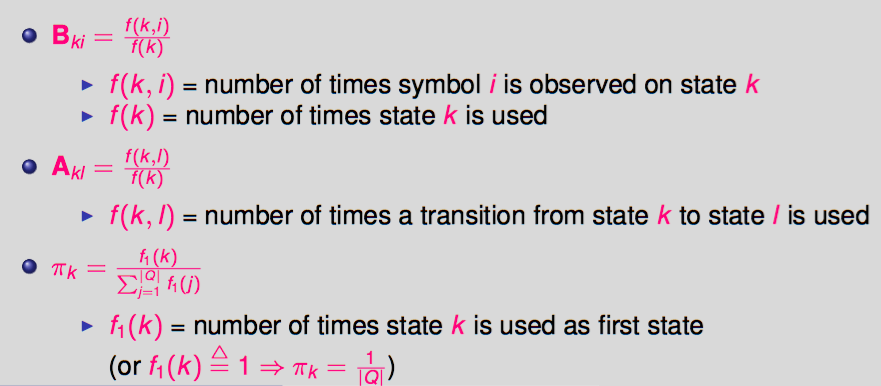
\includegraphics[scale=0.5]{images/29_supervised.png}
 	\caption{Supervised learning.}
\end{figure}

\subsubsection{Unsupervised learning}

The sentences are not annoted. There is two algorithm. The first one is \textbf{Viterbi training}.

\begin{figure}[htp]
	\centering
	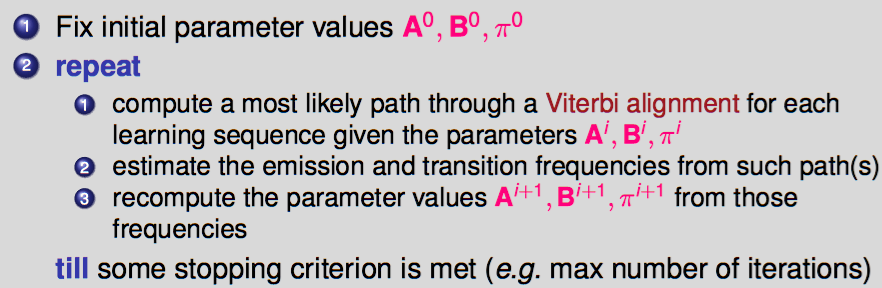
\includegraphics[scale=0.5]{images/30_viterbi.png}
 	\caption{Viterbi learning.}
\end{figure}

The second is \textbf{Forward-Backward} or \textbf{Braaum-Welch} algorithm. Viterbi training is an approximation as it considers that each training sentence is generated along a single path. A more accurate estimation is obtained if one considers all possible paths to generate each sentence.

\begin{itemize}
	\item actual frequencies are replaced by expected frequencies;
	\item   special case of expectation-maximization (EM) procedure
\end{itemize}

Viterbi and Baum-Welch training are both sensitive to parameter initialization.

\subsection{Concrete example}

For CpG islands, we can use a 2-state HMM.

\begin{figure}[htp]
	\centering
	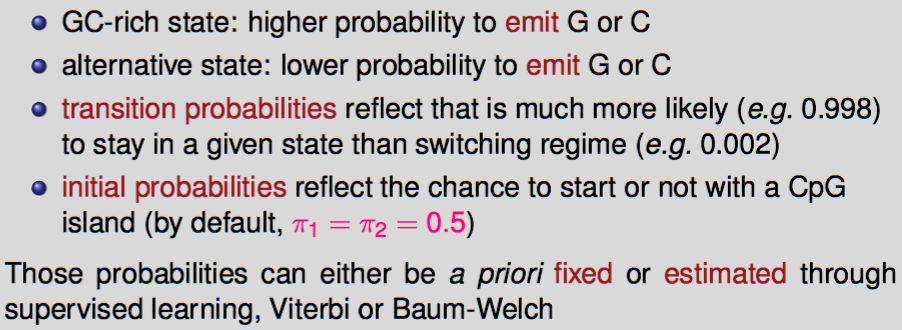
\includegraphics[scale=0.5]{images/31_islands.png}
\end{figure}